\documentclass{standalone}
\usepackage{tikz}
\usetikzlibrary{patterns, positioning}


\begin{document}
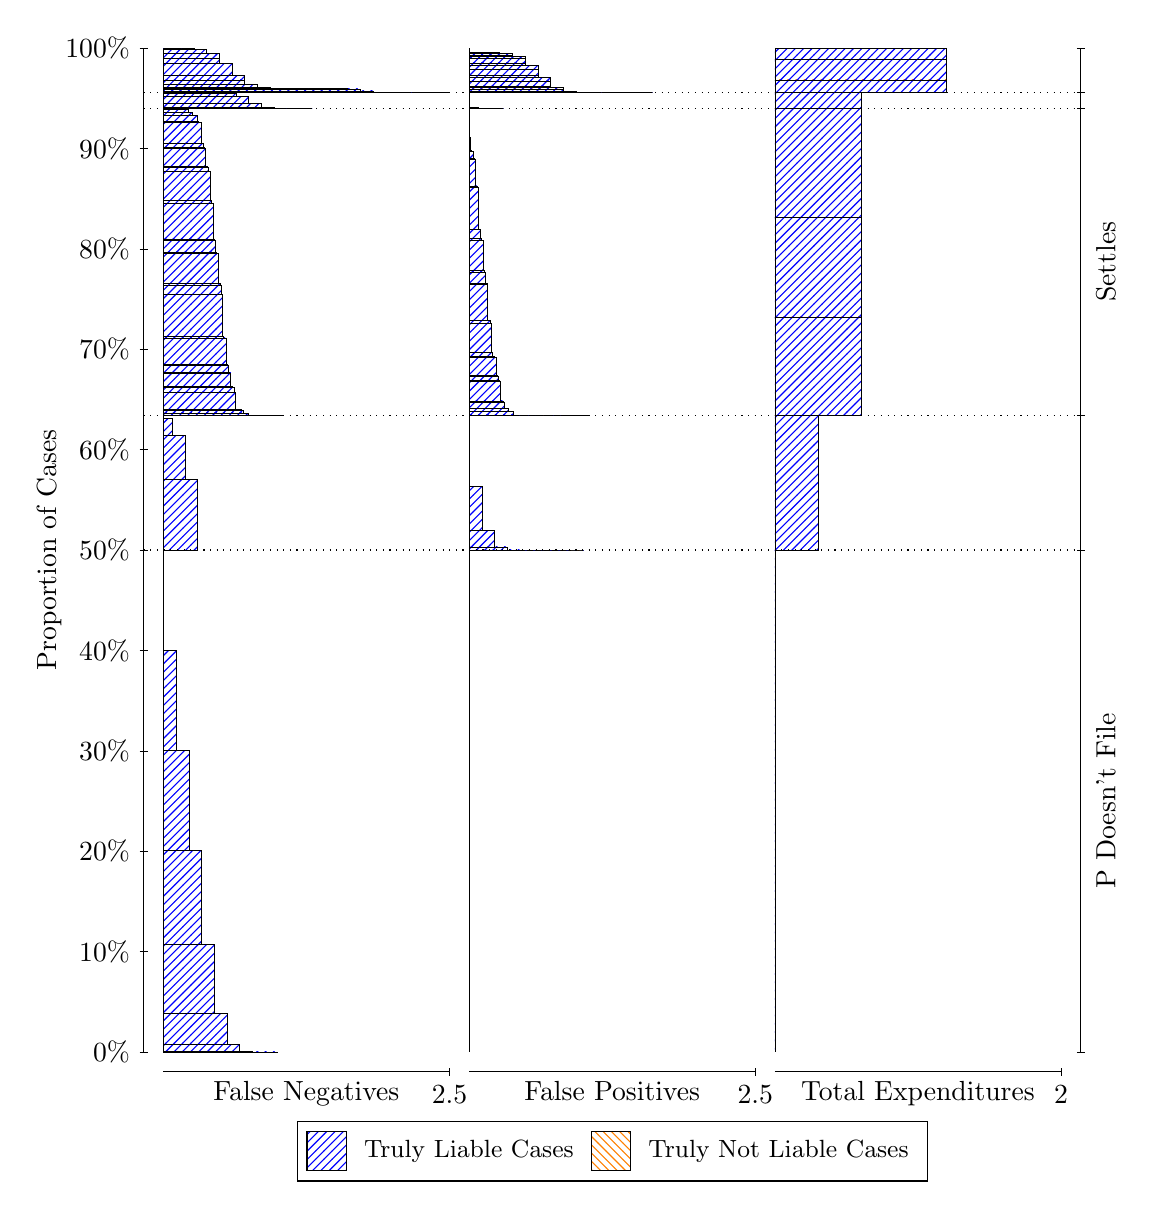
\begin{tikzpicture}
\draw[black, very thin] (1.5,1.75) -- (1.5,14.5);
\node[rotate=90, text=black, anchor=center] at (0.3, 8.125) {Proportion of Cases};
\draw[black, very thin] (1.45,1.75) -- (1.55,1.75);
\node[text=black, anchor=east] at (1.45, 1.75) {0\%};
\draw[black, very thin] (1.45,3.025) -- (1.55,3.025);
\node[text=black, anchor=east] at (1.45, 3.025) {10\%};
\draw[black, very thin] (1.45,4.3) -- (1.55,4.3);
\node[text=black, anchor=east] at (1.45, 4.3) {20\%};
\draw[black, very thin] (1.45,5.575) -- (1.55,5.575);
\node[text=black, anchor=east] at (1.45, 5.575) {30\%};
\draw[black, very thin] (1.45,6.85) -- (1.55,6.85);
\node[text=black, anchor=east] at (1.45, 6.85) {40\%};
\draw[black, very thin] (1.45,8.125) -- (1.55,8.125);
\node[text=black, anchor=east] at (1.45, 8.125) {50\%};
\draw[black, very thin] (1.45,9.4) -- (1.55,9.4);
\node[text=black, anchor=east] at (1.45, 9.4) {60\%};
\draw[black, very thin] (1.45,10.675) -- (1.55,10.675);
\node[text=black, anchor=east] at (1.45, 10.675) {70\%};
\draw[black, very thin] (1.45,11.95) -- (1.55,11.95);
\node[text=black, anchor=east] at (1.45, 11.95) {80\%};
\draw[black, very thin] (1.45,13.225) -- (1.55,13.225);
\node[text=black, anchor=east] at (1.45, 13.225) {90\%};
\draw[black, very thin] (1.45,14.5) -- (1.55,14.5);
\node[text=black, anchor=east] at (1.45, 14.5) {100\%};

\draw[black, very thin] (13.4,1.75) -- (13.4,14.5);
\draw[black, very thin] (13.35,1.75) -- (13.45,1.75);
\node[anchor=west] at (13.35, 1.75) {};
\draw[black, very thin] (13.35,8.125) -- (13.45,8.125);
\node[anchor=west] at (13.35, 8.125) {};
\draw[black, very thin] (13.35,9.8329) -- (13.45,9.8329);
\node[anchor=west] at (13.35, 9.8329) {};
\draw[black, very thin] (13.35,13.737) -- (13.45,13.737);
\node[anchor=west] at (13.35, 13.737) {};
\draw[black, very thin] (13.35,13.933) -- (13.45,13.933);
\node[anchor=west] at (13.35, 13.933) {};
\draw[black, very thin] (13.35,14.5) -- (13.45,14.5);
\node[anchor=west] at (13.35, 14.5) {};

\draw[black, very thin, pattern color=blue, pattern=north east lines] (1.75,1.75) rectangle (3.2033,1.75);
\draw[black, very thin, pattern color=blue, pattern=north east lines] (1.75,1.75) rectangle (3.0419,1.7503);
\draw[black, very thin, pattern color=blue, pattern=north east lines] (1.75,1.7503) rectangle (2.8804,1.7583);
\draw[black, very thin, pattern color=blue, pattern=north east lines] (1.75,1.7583) rectangle (2.7189,1.8435);
\draw[black, very thin, pattern color=blue, pattern=north east lines] (1.75,1.8435) rectangle (2.5574,2.2369);
\draw[black, very thin, pattern color=blue, pattern=north east lines] (1.75,2.2369) rectangle (2.3959,3.1185);
\draw[black, very thin, pattern color=blue, pattern=north east lines] (1.75,3.1185) rectangle (2.2344,4.3083);
\draw[black, very thin, pattern color=blue, pattern=north east lines] (1.75,4.3083) rectangle (2.073,5.5753);
\draw[black, very thin, pattern color=blue, pattern=north east lines] (1.75,5.5753) rectangle (1.9115,6.85);
\draw[black, very thin, pattern color=orange, pattern=north west lines] (1.75,6.85) rectangle (1.75,6.85);
\draw[black, very thin, pattern color=blue, pattern=north east lines] (1.75,6.85) rectangle (1.75,8.125);
\draw[black, very thin, pattern color=blue, pattern=north east lines] (1.75,8.125) rectangle (2.186,9.0243);
\draw[black, very thin, pattern color=blue, pattern=north east lines] (1.75,9.0243) rectangle (2.0245,9.5812);
\draw[black, very thin, pattern color=blue, pattern=north east lines] (1.75,9.5812) rectangle (1.863,9.792);
\draw[black, very thin, pattern color=orange, pattern=north west lines] (1.75,9.792) rectangle (1.75,9.792);
\draw[black, very thin, pattern color=blue, pattern=north east lines] (1.75,9.792) rectangle (1.75,9.8329);
\draw[black, very thin, pattern color=blue, pattern=north east lines] (1.75,9.8329) rectangle (3.276,9.8329);
\draw[black, very thin, pattern color=blue, pattern=north east lines] (1.75,9.8329) rectangle (3.2033,9.8329);
\draw[black, very thin, pattern color=blue, pattern=north east lines] (1.75,9.8329) rectangle (3.1307,9.8329);
\draw[black, very thin, pattern color=blue, pattern=north east lines] (1.75,9.8329) rectangle (3.1145,9.8329);
\draw[black, very thin, pattern color=blue, pattern=north east lines] (1.75,9.8329) rectangle (3.058,9.8329);
\draw[black, very thin, pattern color=blue, pattern=north east lines] (1.75,9.8329) rectangle (3.0419,9.8329);
\draw[black, very thin, pattern color=blue, pattern=north east lines] (1.75,9.8329) rectangle (2.9853,9.8338);
\draw[black, very thin, pattern color=blue, pattern=north east lines] (1.75,9.8338) rectangle (2.9692,9.8339);
\draw[black, very thin, pattern color=blue, pattern=north east lines] (1.75,9.8339) rectangle (2.953,9.834);
\draw[black, very thin, pattern color=blue, pattern=north east lines] (1.75,9.834) rectangle (2.9127,9.834);
\draw[black, very thin, pattern color=blue, pattern=north east lines] (1.75,9.834) rectangle (2.8965,9.8342);
\draw[black, very thin, pattern color=blue, pattern=north east lines] (1.75,9.8342) rectangle (2.8804,9.8343);
\draw[black, very thin, pattern color=blue, pattern=north east lines] (1.75,9.8343) rectangle (2.84,9.8344);
\draw[black, very thin, pattern color=blue, pattern=north east lines] (1.75,9.8344) rectangle (2.8239,9.8592);
\draw[black, very thin, pattern color=blue, pattern=north east lines] (1.75,9.8592) rectangle (2.8077,9.8655);
\draw[black, very thin, pattern color=blue, pattern=north east lines] (1.75,9.8655) rectangle (2.7916,9.8669);
\draw[black, very thin, pattern color=blue, pattern=north east lines] (1.75,9.8669) rectangle (2.7673,9.8954);
\draw[black, very thin, pattern color=blue, pattern=north east lines] (1.75,9.8954) rectangle (2.7512,9.8965);
\draw[black, very thin, pattern color=blue, pattern=north east lines] (1.75,9.8965) rectangle (2.735,9.9067);
\draw[black, very thin, pattern color=blue, pattern=north east lines] (1.75,9.9067) rectangle (2.7189,9.909);
\draw[black, very thin, pattern color=blue, pattern=north east lines] (1.75,9.909) rectangle (2.6785,9.9107);
\draw[black, very thin, pattern color=blue, pattern=north east lines] (1.75,9.9107) rectangle (2.6624,10.132);
\draw[black, very thin, pattern color=blue, pattern=north east lines] (1.75,10.132) rectangle (2.6462,10.188);
\draw[black, very thin, pattern color=blue, pattern=north east lines] (1.75,10.188) rectangle (2.6301,10.202);
\draw[black, very thin, pattern color=blue, pattern=north east lines] (1.75,10.202) rectangle (2.6059,10.373);
\draw[black, very thin, pattern color=blue, pattern=north east lines] (1.75,10.373) rectangle (2.5897,10.383);
\draw[black, very thin, pattern color=blue, pattern=north east lines] (1.75,10.383) rectangle (2.5736,10.469);
\draw[black, very thin, pattern color=blue, pattern=north east lines] (1.75,10.469) rectangle (2.5574,10.483);
\draw[black, very thin, pattern color=blue, pattern=north east lines] (1.75,10.483) rectangle (2.5493,10.819);
\draw[black, very thin, pattern color=blue, pattern=north east lines] (1.75,10.819) rectangle (2.517,10.837);
\draw[black, very thin, pattern color=blue, pattern=north east lines] (1.75,10.837) rectangle (2.5009,11.37);
\draw[black, very thin, pattern color=blue, pattern=north east lines] (1.75,11.37) rectangle (2.4847,11.484);
\draw[black, very thin, pattern color=blue, pattern=north east lines] (1.75,11.484) rectangle (2.4686,11.511);
\draw[black, very thin, pattern color=blue, pattern=north east lines] (1.75,11.511) rectangle (2.4444,11.89);
\draw[black, very thin, pattern color=blue, pattern=north east lines] (1.75,11.89) rectangle (2.4282,11.912);
\draw[black, very thin, pattern color=blue, pattern=north east lines] (1.75,11.912) rectangle (2.4121,12.061);
\draw[black, very thin, pattern color=blue, pattern=north east lines] (1.75,12.061) rectangle (2.3959,12.075);
\draw[black, very thin, pattern color=blue, pattern=north east lines] (1.75,12.075) rectangle (2.3879,12.528);
\draw[black, very thin, pattern color=blue, pattern=north east lines] (1.75,12.528) rectangle (2.3556,12.565);
\draw[black, very thin, pattern color=blue, pattern=north east lines] (1.75,12.565) rectangle (2.3394,12.931);
\draw[black, very thin, pattern color=blue, pattern=north east lines] (1.75,12.931) rectangle (2.3233,12.989);
\draw[black, very thin, pattern color=blue, pattern=north east lines] (1.75,12.989) rectangle (2.3071,12.999);
\draw[black, very thin, pattern color=blue, pattern=north east lines] (1.75,12.999) rectangle (2.2829,13.228);
\draw[black, very thin, pattern color=blue, pattern=north east lines] (1.75,13.228) rectangle (2.2667,13.236);
\draw[black, very thin, pattern color=blue, pattern=north east lines] (1.75,13.236) rectangle (2.2506,13.293);
\draw[black, very thin, pattern color=blue, pattern=north east lines] (1.75,13.293) rectangle (2.2344,13.295);
\draw[black, very thin, pattern color=blue, pattern=north east lines] (1.75,13.295) rectangle (2.2264,13.551);
\draw[black, very thin, pattern color=blue, pattern=north east lines] (1.75,13.551) rectangle (2.1941,13.565);
\draw[black, very thin, pattern color=blue, pattern=north east lines] (1.75,13.565) rectangle (2.1779,13.641);
\draw[black, very thin, pattern color=blue, pattern=north east lines] (1.75,13.641) rectangle (2.1618,13.648);
\draw[black, very thin, pattern color=blue, pattern=north east lines] (1.75,13.648) rectangle (2.1456,13.649);
\draw[black, very thin, pattern color=blue, pattern=north east lines] (1.75,13.649) rectangle (2.1214,13.682);
\draw[black, very thin, pattern color=blue, pattern=north east lines] (1.75,13.682) rectangle (2.1053,13.682);
\draw[black, very thin, pattern color=blue, pattern=north east lines] (1.75,13.682) rectangle (2.0891,13.687);
\draw[black, very thin, pattern color=blue, pattern=north east lines] (1.75,13.687) rectangle (2.073,13.687);
\draw[black, very thin, pattern color=blue, pattern=north east lines] (1.75,13.687) rectangle (2.0649,13.728);
\draw[black, very thin, pattern color=blue, pattern=north east lines] (1.75,13.728) rectangle (2.0326,13.729);
\draw[black, very thin, pattern color=blue, pattern=north east lines] (1.75,13.729) rectangle (2.0164,13.734);
\draw[black, very thin, pattern color=blue, pattern=north east lines] (1.75,13.734) rectangle (2.0003,13.734);
\draw[black, very thin, pattern color=blue, pattern=north east lines] (1.75,13.734) rectangle (1.9841,13.734);
\draw[black, very thin, pattern color=blue, pattern=north east lines] (1.75,13.734) rectangle (1.9599,13.735);
\draw[black, very thin, pattern color=blue, pattern=north east lines] (1.75,13.735) rectangle (1.9438,13.735);
\draw[black, very thin, pattern color=blue, pattern=north east lines] (1.75,13.735) rectangle (1.9276,13.735);
\draw[black, very thin, pattern color=blue, pattern=north east lines] (1.75,13.735) rectangle (1.9115,13.735);
\draw[black, very thin, pattern color=blue, pattern=north east lines] (1.75,13.735) rectangle (1.9034,13.737);
\draw[black, very thin, pattern color=blue, pattern=north east lines] (1.75,13.737) rectangle (1.8711,13.737);
\draw[black, very thin, pattern color=blue, pattern=north east lines] (1.75,13.737) rectangle (1.855,13.737);
\draw[black, very thin, pattern color=blue, pattern=north east lines] (1.75,13.737) rectangle (1.8388,13.737);
\draw[black, very thin, pattern color=blue, pattern=north east lines] (1.75,13.737) rectangle (1.8227,13.737);
\draw[black, very thin, pattern color=blue, pattern=north east lines] (1.75,13.737) rectangle (1.7984,13.737);
\draw[black, very thin, pattern color=blue, pattern=north east lines] (1.75,13.737) rectangle (1.7823,13.737);
\draw[black, very thin, pattern color=blue, pattern=north east lines] (1.75,13.737) rectangle (1.7661,13.737);
\draw[black, very thin, pattern color=orange, pattern=north west lines] (1.75,13.737) rectangle (1.75,13.737);
\draw[black, very thin, pattern color=blue, pattern=north east lines] (1.75,13.737) rectangle (1.75,13.737);
\draw[black, very thin, pattern color=blue, pattern=north east lines] (1.75,13.737) rectangle (3.6393,13.737);
\draw[black, very thin, pattern color=blue, pattern=north east lines] (1.75,13.737) rectangle (3.4779,13.737);
\draw[black, very thin, pattern color=blue, pattern=north east lines] (1.75,13.737) rectangle (3.3164,13.737);
\draw[black, very thin, pattern color=blue, pattern=north east lines] (1.75,13.737) rectangle (3.1549,13.743);
\draw[black, very thin, pattern color=blue, pattern=north east lines] (1.75,13.743) rectangle (2.9934,13.795);
\draw[black, very thin, pattern color=blue, pattern=north east lines] (1.75,13.795) rectangle (2.8319,13.887);
\draw[black, very thin, pattern color=blue, pattern=north east lines] (1.75,13.887) rectangle (2.6704,13.927);
\draw[black, very thin, pattern color=blue, pattern=north east lines] (1.75,13.927) rectangle (2.509,13.933);
\draw[black, very thin, pattern color=blue, pattern=north east lines] (1.75,13.933) rectangle (2.3475,13.933);
\draw[black, very thin, pattern color=blue, pattern=north east lines] (1.75,13.933) rectangle (2.186,13.933);
\draw[black, very thin, pattern color=orange, pattern=north west lines] (1.75,13.933) rectangle (1.75,13.933);
\draw[black, very thin, pattern color=blue, pattern=north east lines] (1.75,13.933) rectangle (5.3833,13.933);
\draw[black, very thin, pattern color=blue, pattern=north east lines] (1.75,13.933) rectangle (5.2219,13.933);
\draw[black, very thin, pattern color=blue, pattern=north east lines] (1.75,13.933) rectangle (5.0604,13.933);
\draw[black, very thin, pattern color=blue, pattern=north east lines] (1.75,13.933) rectangle (4.8989,13.933);
\draw[black, very thin, pattern color=blue, pattern=north east lines] (1.75,13.933) rectangle (4.8989,13.933);
\draw[black, very thin, pattern color=blue, pattern=north east lines] (1.75,13.933) rectangle (4.7374,13.934);
\draw[black, very thin, pattern color=blue, pattern=north east lines] (1.75,13.934) rectangle (4.5759,13.935);
\draw[black, very thin, pattern color=blue, pattern=north east lines] (1.75,13.935) rectangle (4.5759,13.937);
\draw[black, very thin, pattern color=blue, pattern=north east lines] (1.75,13.937) rectangle (4.5759,13.938);
\draw[black, very thin, pattern color=blue, pattern=north east lines] (1.75,13.938) rectangle (4.4144,13.949);
\draw[black, very thin, pattern color=blue, pattern=north east lines] (1.75,13.949) rectangle (4.4144,13.956);
\draw[black, very thin, pattern color=blue, pattern=north east lines] (1.75,13.956) rectangle (4.253,13.974);
\draw[black, very thin, pattern color=blue, pattern=north east lines] (1.75,13.974) rectangle (4.253,13.982);
\draw[black, very thin, pattern color=blue, pattern=north east lines] (1.75,13.982) rectangle (4.0915,13.989);
\draw[black, very thin, pattern color=blue, pattern=north east lines] (1.75,13.989) rectangle (4.0915,13.991);
\draw[black, very thin, pattern color=blue, pattern=north east lines] (1.75,13.991) rectangle (3.93,13.992);
\draw[black, very thin, pattern color=blue, pattern=north east lines] (1.75,13.992) rectangle (3.7685,13.992);
\draw[black, very thin, pattern color=blue, pattern=north east lines] (1.75,13.992) rectangle (3.7524,13.992);
\draw[black, very thin, pattern color=blue, pattern=north east lines] (1.75,13.992) rectangle (3.607,13.992);
\draw[black, very thin, pattern color=blue, pattern=north east lines] (1.75,13.992) rectangle (3.607,13.992);
\draw[black, very thin, pattern color=blue, pattern=north east lines] (1.75,13.992) rectangle (3.5909,13.992);
\draw[black, very thin, pattern color=blue, pattern=north east lines] (1.75,13.992) rectangle (3.4456,13.992);
\draw[black, very thin, pattern color=blue, pattern=north east lines] (1.75,13.992) rectangle (3.4294,13.992);
\draw[black, very thin, pattern color=blue, pattern=north east lines] (1.75,13.992) rectangle (3.2841,13.992);
\draw[black, very thin, pattern color=blue, pattern=north east lines] (1.75,13.992) rectangle (3.2679,13.992);
\draw[black, very thin, pattern color=blue, pattern=north east lines] (1.75,13.992) rectangle (3.2679,13.992);
\draw[black, very thin, pattern color=blue, pattern=north east lines] (1.75,13.992) rectangle (3.1064,13.994);
\draw[black, very thin, pattern color=blue, pattern=north east lines] (1.75,13.994) rectangle (3.1064,13.997);
\draw[black, very thin, pattern color=blue, pattern=north east lines] (1.75,13.997) rectangle (2.945,14.037);
\draw[black, very thin, pattern color=blue, pattern=north east lines] (1.75,14.037) rectangle (2.7835,14.096);
\draw[black, very thin, pattern color=blue, pattern=north east lines] (1.75,14.096) rectangle (2.7835,14.153);
\draw[black, very thin, pattern color=blue, pattern=north east lines] (1.75,14.153) rectangle (2.622,14.308);
\draw[black, very thin, pattern color=blue, pattern=north east lines] (1.75,14.308) rectangle (2.4605,14.366);
\draw[black, very thin, pattern color=blue, pattern=north east lines] (1.75,14.366) rectangle (2.4605,14.37);
\draw[black, very thin, pattern color=blue, pattern=north east lines] (1.75,14.37) rectangle (2.4605,14.43);
\draw[black, very thin, pattern color=blue, pattern=north east lines] (1.75,14.43) rectangle (2.299,14.484);
\draw[black, very thin, pattern color=blue, pattern=north east lines] (1.75,14.484) rectangle (2.299,14.485);
\draw[black, very thin, pattern color=blue, pattern=north east lines] (1.75,14.485) rectangle (2.1376,14.49);
\draw[black, very thin, pattern color=blue, pattern=north east lines] (1.75,14.49) rectangle (2.1376,14.49);
\draw[black, very thin, pattern color=blue, pattern=north east lines] (1.75,14.49) rectangle (2.1376,14.498);
\draw[black, very thin, pattern color=blue, pattern=north east lines] (1.75,14.498) rectangle (1.9761,14.5);
\draw[black, very thin, pattern color=blue, pattern=north east lines] (1.75,14.5) rectangle (1.9761,14.5);
\draw[black, very thin, pattern color=blue, pattern=north east lines] (1.75,14.5) rectangle (1.8146,14.5);
\draw[black, very thin, pattern color=blue, pattern=north east lines] (1.75,14.5) rectangle (1.8146,14.5);
\draw[black, very thin, pattern color=orange, pattern=north west lines] (1.75,14.5) rectangle (1.75,14.5);
\draw[black, very thin, pattern color=blue, pattern=north east lines] (1.75,14.5) rectangle (1.75,14.5);
\draw[black, very thin, pattern color=orange, pattern=north west lines] (5.6333,1.75) rectangle (5.6333,1.75);
\draw[black, very thin, pattern color=blue, pattern=north east lines] (5.6333,1.75) rectangle (5.6333,8.125);
\draw[black, very thin, pattern color=orange, pattern=north west lines] (5.6333,8.125) rectangle (7.0867,8.125);
\draw[black, very thin, pattern color=blue, pattern=north east lines] (5.6333,8.125) rectangle (7.0867,8.125);
\draw[black, very thin, pattern color=blue, pattern=north east lines] (5.6333,8.125) rectangle (6.9252,8.125);
\draw[black, very thin, pattern color=blue, pattern=north east lines] (5.6333,8.125) rectangle (6.7637,8.125);
\draw[black, very thin, pattern color=blue, pattern=north east lines] (5.6333,8.125) rectangle (6.6022,8.125);
\draw[black, very thin, pattern color=blue, pattern=north east lines] (5.6333,8.125) rectangle (6.4407,8.125);
\draw[black, very thin, pattern color=blue, pattern=north east lines] (5.6333,8.125) rectangle (6.2793,8.1275);
\draw[black, very thin, pattern color=blue, pattern=north east lines] (5.6333,8.1275) rectangle (6.1178,8.1659);
\draw[black, very thin, pattern color=blue, pattern=north east lines] (5.6333,8.1659) rectangle (5.9563,8.3767);
\draw[black, very thin, pattern color=blue, pattern=north east lines] (5.6333,8.3767) rectangle (5.7948,8.9336);
\draw[black, very thin, pattern color=blue, pattern=north east lines] (5.6333,8.9336) rectangle (5.6333,9.8329);
\draw[black, very thin, pattern color=orange, pattern=north west lines] (5.6333,9.8329) rectangle (7.1593,9.8329);
\draw[black, very thin, pattern color=blue, pattern=north east lines] (5.6333,9.8329) rectangle (7.1593,9.8329);
\draw[black, very thin, pattern color=blue, pattern=north east lines] (5.6333,9.8329) rectangle (6.9979,9.8329);
\draw[black, very thin, pattern color=orange, pattern=north west lines] (5.6333,9.8329) rectangle (6.9413,9.8329);
\draw[black, very thin, pattern color=blue, pattern=north east lines] (5.6333,9.8329) rectangle (6.9413,9.8329);
\draw[black, very thin, pattern color=orange, pattern=north west lines] (5.6333,9.8329) rectangle (6.8687,9.8329);
\draw[black, very thin, pattern color=blue, pattern=north east lines] (5.6333,9.8329) rectangle (6.8687,9.8329);
\draw[black, very thin, pattern color=blue, pattern=north east lines] (5.6333,9.8329) rectangle (6.8364,9.8329);
\draw[black, very thin, pattern color=orange, pattern=north west lines] (5.6333,9.8329) rectangle (6.796,9.8329);
\draw[black, very thin, pattern color=blue, pattern=north east lines] (5.6333,9.8329) rectangle (6.796,9.8329);
\draw[black, very thin, pattern color=blue, pattern=north east lines] (5.6333,9.8329) rectangle (6.7799,9.8329);
\draw[black, very thin, pattern color=orange, pattern=north west lines] (5.6333,9.8329) rectangle (6.7233,9.8329);
\draw[black, very thin, pattern color=blue, pattern=north east lines] (5.6333,9.8329) rectangle (6.7233,9.8329);
\draw[black, very thin, pattern color=blue, pattern=north east lines] (5.6333,9.8329) rectangle (6.7072,9.8329);
\draw[black, very thin, pattern color=blue, pattern=north east lines] (5.6333,9.8329) rectangle (6.6749,9.8329);
\draw[black, very thin, pattern color=orange, pattern=north west lines] (5.6333,9.8329) rectangle (6.6507,9.8329);
\draw[black, very thin, pattern color=blue, pattern=north east lines] (5.6333,9.8329) rectangle (6.6507,9.8329);
\draw[black, very thin, pattern color=blue, pattern=north east lines] (5.6333,9.8329) rectangle (6.6345,9.8329);
\draw[black, very thin, pattern color=blue, pattern=north east lines] (5.6333,9.8329) rectangle (6.6184,9.8329);
\draw[black, very thin, pattern color=orange, pattern=north west lines] (5.6333,9.8329) rectangle (6.578,9.8329);
\draw[black, very thin, pattern color=blue, pattern=north east lines] (5.6333,9.8329) rectangle (6.578,9.8329);
\draw[black, very thin, pattern color=blue, pattern=north east lines] (5.6333,9.8329) rectangle (6.5619,9.8329);
\draw[black, very thin, pattern color=blue, pattern=north east lines] (5.6333,9.8329) rectangle (6.5457,9.8329);
\draw[black, very thin, pattern color=blue, pattern=north east lines] (5.6333,9.8329) rectangle (6.5134,9.8329);
\draw[black, very thin, pattern color=orange, pattern=north west lines] (5.6333,9.8329) rectangle (6.5053,9.8329);
\draw[black, very thin, pattern color=blue, pattern=north east lines] (5.6333,9.8329) rectangle (6.5053,9.8329);
\draw[black, very thin, pattern color=blue, pattern=north east lines] (5.6333,9.8329) rectangle (6.4892,9.8329);
\draw[black, very thin, pattern color=blue, pattern=north east lines] (5.6333,9.8329) rectangle (6.473,9.8329);
\draw[black, very thin, pattern color=blue, pattern=north east lines] (5.6333,9.8329) rectangle (6.4569,9.8329);
\draw[black, very thin, pattern color=orange, pattern=north west lines] (5.6333,9.8329) rectangle (6.4327,9.8329);
\draw[black, very thin, pattern color=blue, pattern=north east lines] (5.6333,9.8329) rectangle (6.4327,9.8329);
\draw[black, very thin, pattern color=blue, pattern=north east lines] (5.6333,9.8329) rectangle (6.4165,9.8329);
\draw[black, very thin, pattern color=blue, pattern=north east lines] (5.6333,9.8329) rectangle (6.4004,9.833);
\draw[black, very thin, pattern color=blue, pattern=north east lines] (5.6333,9.833) rectangle (6.3842,9.833);
\draw[black, very thin, pattern color=blue, pattern=north east lines] (5.6333,9.833) rectangle (6.3519,9.8345);
\draw[black, very thin, pattern color=blue, pattern=north east lines] (5.6333,9.8345) rectangle (6.3439,9.8345);
\draw[black, very thin, pattern color=blue, pattern=north east lines] (5.6333,9.8345) rectangle (6.3277,9.8346);
\draw[black, very thin, pattern color=blue, pattern=north east lines] (5.6333,9.8346) rectangle (6.3116,9.8346);
\draw[black, very thin, pattern color=blue, pattern=north east lines] (5.6333,9.8346) rectangle (6.2954,9.8357);
\draw[black, very thin, pattern color=blue, pattern=north east lines] (5.6333,9.8357) rectangle (6.2712,9.8357);
\draw[black, very thin, pattern color=blue, pattern=north east lines] (5.6333,9.8357) rectangle (6.255,9.8358);
\draw[black, very thin, pattern color=blue, pattern=north east lines] (5.6333,9.8358) rectangle (6.2389,9.8405);
\draw[black, very thin, pattern color=blue, pattern=north east lines] (5.6333,9.8405) rectangle (6.2227,9.8413);
\draw[black, very thin, pattern color=blue, pattern=north east lines] (5.6333,9.8413) rectangle (6.1904,9.8823);
\draw[black, very thin, pattern color=blue, pattern=north east lines] (5.6333,9.8823) rectangle (6.1824,9.8824);
\draw[black, very thin, pattern color=blue, pattern=north east lines] (5.6333,9.8824) rectangle (6.1662,9.8873);
\draw[black, very thin, pattern color=blue, pattern=north east lines] (5.6333,9.8873) rectangle (6.1501,9.8878);
\draw[black, very thin, pattern color=blue, pattern=north east lines] (5.6333,9.8878) rectangle (6.1339,9.921);
\draw[black, very thin, pattern color=blue, pattern=north east lines] (5.6333,9.921) rectangle (6.1097,9.9217);
\draw[black, very thin, pattern color=blue, pattern=north east lines] (5.6333,9.9217) rectangle (6.0936,9.9284);
\draw[black, very thin, pattern color=blue, pattern=north east lines] (5.6333,9.9284) rectangle (6.0774,10.005);
\draw[black, very thin, pattern color=blue, pattern=north east lines] (5.6333,10.005) rectangle (6.0613,10.018);
\draw[black, very thin, pattern color=blue, pattern=north east lines] (5.6333,10.018) rectangle (6.029,10.274);
\draw[black, very thin, pattern color=blue, pattern=north east lines] (5.6333,10.274) rectangle (6.0209,10.277);
\draw[black, very thin, pattern color=blue, pattern=north east lines] (5.6333,10.277) rectangle (6.0047,10.334);
\draw[black, very thin, pattern color=blue, pattern=north east lines] (5.6333,10.334) rectangle (5.9886,10.342);
\draw[black, very thin, pattern color=blue, pattern=north east lines] (5.6333,10.342) rectangle (5.9724,10.57);
\draw[black, very thin, pattern color=blue, pattern=north east lines] (5.6333,10.57) rectangle (5.9482,10.581);
\draw[black, very thin, pattern color=blue, pattern=north east lines] (5.6333,10.581) rectangle (5.9321,10.639);
\draw[black, very thin, pattern color=blue, pattern=north east lines] (5.6333,10.639) rectangle (5.9159,11.005);
\draw[black, very thin, pattern color=blue, pattern=north east lines] (5.6333,11.005) rectangle (5.8998,11.042);
\draw[black, very thin, pattern color=blue, pattern=north east lines] (5.6333,11.042) rectangle (5.8675,11.495);
\draw[black, very thin, pattern color=blue, pattern=north east lines] (5.6333,11.495) rectangle (5.8594,11.509);
\draw[black, very thin, pattern color=blue, pattern=north east lines] (5.6333,11.509) rectangle (5.8433,11.658);
\draw[black, very thin, pattern color=blue, pattern=north east lines] (5.6333,11.658) rectangle (5.8271,11.68);
\draw[black, very thin, pattern color=blue, pattern=north east lines] (5.6333,11.68) rectangle (5.811,12.059);
\draw[black, very thin, pattern color=blue, pattern=north east lines] (5.6333,12.059) rectangle (5.7867,12.085);
\draw[black, very thin, pattern color=blue, pattern=north east lines] (5.6333,12.085) rectangle (5.7706,12.199);
\draw[black, very thin, pattern color=blue, pattern=north east lines] (5.6333,12.199) rectangle (5.7544,12.733);
\draw[black, very thin, pattern color=blue, pattern=north east lines] (5.6333,12.733) rectangle (5.7383,12.75);
\draw[black, very thin, pattern color=blue, pattern=north east lines] (5.6333,12.75) rectangle (5.706,13.086);
\draw[black, very thin, pattern color=blue, pattern=north east lines] (5.6333,13.086) rectangle (5.6979,13.1);
\draw[black, very thin, pattern color=blue, pattern=north east lines] (5.6333,13.1) rectangle (5.6818,13.186);
\draw[black, very thin, pattern color=blue, pattern=north east lines] (5.6333,13.186) rectangle (5.6656,13.197);
\draw[black, very thin, pattern color=blue, pattern=north east lines] (5.6333,13.197) rectangle (5.6495,13.368);
\draw[black, very thin, pattern color=blue, pattern=north east lines] (5.6333,13.368) rectangle (5.6333,13.737);
\draw[black, very thin, pattern color=orange, pattern=north west lines] (5.6333,13.737) rectangle (6.0693,13.737);
\draw[black, very thin, pattern color=blue, pattern=north east lines] (5.6333,13.737) rectangle (6.0693,13.737);
\draw[black, very thin, pattern color=blue, pattern=north east lines] (5.6333,13.737) rectangle (5.9079,13.737);
\draw[black, very thin, pattern color=blue, pattern=north east lines] (5.6333,13.737) rectangle (5.7464,13.742);
\draw[black, very thin, pattern color=blue, pattern=north east lines] (5.6333,13.742) rectangle (5.6333,13.933);
\draw[black, very thin, pattern color=orange, pattern=north west lines] (5.6333,13.933) rectangle (7.9587,13.933);
\draw[black, very thin, pattern color=blue, pattern=north east lines] (5.6333,13.933) rectangle (7.9587,13.933);
\draw[black, very thin, pattern color=orange, pattern=north west lines] (5.6333,13.933) rectangle (7.7972,13.933);
\draw[black, very thin, pattern color=blue, pattern=north east lines] (5.6333,13.933) rectangle (7.7972,13.933);
\draw[black, very thin, pattern color=orange, pattern=north west lines] (5.6333,13.933) rectangle (7.6357,13.933);
\draw[black, very thin, pattern color=blue, pattern=north east lines] (5.6333,13.933) rectangle (7.6357,13.933);
\draw[black, very thin, pattern color=blue, pattern=north east lines] (5.6333,13.933) rectangle (7.4742,13.933);
\draw[black, very thin, pattern color=orange, pattern=north west lines] (5.6333,13.933) rectangle (7.4742,13.933);
\draw[black, very thin, pattern color=blue, pattern=north east lines] (5.6333,13.933) rectangle (7.4742,13.933);
\draw[black, very thin, pattern color=blue, pattern=north east lines] (5.6333,13.933) rectangle (7.3127,13.933);
\draw[black, very thin, pattern color=orange, pattern=north west lines] (5.6333,13.933) rectangle (7.3127,13.933);
\draw[black, very thin, pattern color=blue, pattern=north east lines] (5.6333,13.933) rectangle (7.3127,13.933);
\draw[black, very thin, pattern color=blue, pattern=north east lines] (5.6333,13.933) rectangle (7.1513,13.935);
\draw[black, very thin, pattern color=orange, pattern=north west lines] (5.6333,13.935) rectangle (7.1513,13.935);
\draw[black, very thin, pattern color=blue, pattern=north east lines] (5.6333,13.935) rectangle (7.1513,13.935);
\draw[black, very thin, pattern color=blue, pattern=north east lines] (5.6333,13.935) rectangle (6.9898,13.94);
\draw[black, very thin, pattern color=orange, pattern=north west lines] (5.6333,13.94) rectangle (6.9898,13.94);
\draw[black, very thin, pattern color=blue, pattern=north east lines] (5.6333,13.94) rectangle (6.9898,13.948);
\draw[black, very thin, pattern color=blue, pattern=north east lines] (5.6333,13.948) rectangle (6.9898,13.948);
\draw[black, very thin, pattern color=blue, pattern=north east lines] (5.6333,13.948) rectangle (6.9898,13.948);
\draw[black, very thin, pattern color=blue, pattern=north east lines] (5.6333,13.948) rectangle (6.8283,13.981);
\draw[black, very thin, pattern color=orange, pattern=north west lines] (5.6333,13.981) rectangle (6.8283,13.981);
\draw[black, very thin, pattern color=blue, pattern=north east lines] (5.6333,13.981) rectangle (6.8283,14.003);
\draw[black, very thin, pattern color=blue, pattern=north east lines] (5.6333,14.003) rectangle (6.8283,14.003);
\draw[black, very thin, pattern color=blue, pattern=north east lines] (5.6333,14.003) rectangle (6.6668,14.02);
\draw[black, very thin, pattern color=blue, pattern=north east lines] (5.6333,14.02) rectangle (6.6668,14.083);
\draw[black, very thin, pattern color=blue, pattern=north east lines] (5.6333,14.083) rectangle (6.6668,14.125);
\draw[black, very thin, pattern color=blue, pattern=north east lines] (5.6333,14.125) rectangle (6.5053,14.154);
\draw[black, very thin, pattern color=blue, pattern=north east lines] (5.6333,14.154) rectangle (6.5053,14.233);
\draw[black, very thin, pattern color=blue, pattern=north east lines] (5.6333,14.233) rectangle (6.5053,14.28);
\draw[black, very thin, pattern color=blue, pattern=north east lines] (5.6333,14.28) rectangle (6.3439,14.311);
\draw[black, very thin, pattern color=blue, pattern=north east lines] (5.6333,14.311) rectangle (6.3439,14.312);
\draw[black, very thin, pattern color=blue, pattern=north east lines] (5.6333,14.312) rectangle (6.3439,14.375);
\draw[black, very thin, pattern color=blue, pattern=north east lines] (5.6333,14.375) rectangle (6.3439,14.396);
\draw[black, very thin, pattern color=blue, pattern=north east lines] (5.6333,14.396) rectangle (6.1824,14.413);
\draw[black, very thin, pattern color=blue, pattern=north east lines] (5.6333,14.413) rectangle (6.1824,14.436);
\draw[black, very thin, pattern color=blue, pattern=north east lines] (5.6333,14.436) rectangle (6.0209,14.437);
\draw[black, very thin, pattern color=blue, pattern=north east lines] (5.6333,14.437) rectangle (6.0209,14.441);
\draw[black, very thin, pattern color=blue, pattern=north east lines] (5.6333,14.441) rectangle (6.0209,14.441);
\draw[black, very thin, pattern color=blue, pattern=north east lines] (5.6333,14.441) rectangle (5.8594,14.441);
\draw[black, very thin, pattern color=blue, pattern=north east lines] (5.6333,14.441) rectangle (5.8594,14.441);
\draw[black, very thin, pattern color=orange, pattern=north west lines] (5.6333,14.441) rectangle (5.8433,14.441);
\draw[black, very thin, pattern color=blue, pattern=north east lines] (5.6333,14.441) rectangle (5.8433,14.441);
\draw[black, very thin, pattern color=blue, pattern=north east lines] (5.6333,14.441) rectangle (5.6979,14.441);
\draw[black, very thin, pattern color=blue, pattern=north east lines] (5.6333,14.441) rectangle (5.6979,14.441);
\draw[black, very thin, pattern color=blue, pattern=north east lines] (5.6333,14.441) rectangle (5.6979,14.441);
\draw[black, very thin, pattern color=orange, pattern=north west lines] (5.6333,14.441) rectangle (5.6818,14.441);
\draw[black, very thin, pattern color=blue, pattern=north east lines] (5.6333,14.441) rectangle (5.6818,14.441);
\draw[black, very thin, pattern color=orange, pattern=north west lines] (5.6333,14.441) rectangle (5.6333,14.441);
\draw[black, very thin, pattern color=blue, pattern=north east lines] (5.6333,14.441) rectangle (5.6333,14.5);
\draw[black, very thin, pattern color=orange, pattern=north west lines] (9.5167,1.75) rectangle (9.5167,1.75);
\draw[black, very thin, pattern color=blue, pattern=north east lines] (9.5167,1.75) rectangle (9.5167,8.125);
\draw[black, very thin, pattern color=orange, pattern=north west lines] (9.5167,8.125) rectangle (10.062,8.125);
\draw[black, very thin, pattern color=blue, pattern=north east lines] (9.5167,8.125) rectangle (10.062,9.8329);
\draw[black, very thin, pattern color=orange, pattern=north west lines] (9.5167,9.8329) rectangle (10.607,9.8329);
\draw[black, very thin, pattern color=blue, pattern=north east lines] (9.5167,9.8329) rectangle (10.607,11.086);
\draw[black, very thin, pattern color=orange, pattern=north west lines] (9.5167,11.086) rectangle (10.607,11.086);
\draw[black, very thin, pattern color=blue, pattern=north east lines] (9.5167,11.086) rectangle (10.607,12.347);
\draw[black, very thin, pattern color=orange, pattern=north west lines] (9.5167,12.347) rectangle (10.607,12.347);
\draw[black, very thin, pattern color=blue, pattern=north east lines] (9.5167,12.347) rectangle (10.607,13.737);
\draw[black, very thin, pattern color=orange, pattern=north west lines] (9.5167,13.737) rectangle (10.607,13.737);
\draw[black, very thin, pattern color=blue, pattern=north east lines] (9.5167,13.737) rectangle (10.607,13.933);
\draw[black, very thin, pattern color=orange, pattern=north west lines] (9.5167,13.933) rectangle (11.697,13.933);
\draw[black, very thin, pattern color=blue, pattern=north east lines] (9.5167,13.933) rectangle (11.697,14.096);
\draw[black, very thin, pattern color=orange, pattern=north west lines] (9.5167,14.096) rectangle (11.697,14.096);
\draw[black, very thin, pattern color=blue, pattern=north east lines] (9.5167,14.096) rectangle (11.697,14.358);
\draw[black, very thin, pattern color=orange, pattern=north west lines] (9.5167,14.358) rectangle (11.697,14.358);
\draw[black, very thin, pattern color=blue, pattern=north east lines] (9.5167,14.358) rectangle (11.697,14.5);
\draw[black, dotted] (1.5,8.125) -- (13.4,8.125);
\draw[black, dotted] (1.5,9.8329) -- (13.4,9.8329);
\draw[black, dotted] (1.5,13.737) -- (13.4,13.737);
\draw[black, dotted] (1.5,13.933) -- (13.4,13.933);
\draw[black, very thin] (1.75,1.5) -- (5.3833,1.5);
\node[text=black, anchor=north] at (3.5667, 1.5) {False Negatives};
\draw[black, very thin] (5.3833,1.45) -- (5.3833,1.55);
\node[text=black, anchor=north] at (5.3833, 1.45) {2.5};

\draw[black, very thin] (5.6333,1.5) -- (9.2667,1.5);
\node[text=black, anchor=north] at (7.45, 1.5) {False Positives};
\draw[black, very thin] (9.2667,1.45) -- (9.2667,1.55);
\node[text=black, anchor=north] at (9.2667, 1.45) {2.5};

\draw[black, very thin] (9.5167,1.5) -- (13.15,1.5);
\node[text=black, anchor=north] at (11.333, 1.5) {Total Expenditures};
\draw[black, very thin] (13.15,1.45) -- (13.15,1.55);
\node[text=black, anchor=north] at (13.15, 1.45) {2};

\node[text=black, centered, rotate=90] at (13.72, 4.9375) {P Doesn't File};

\node[text=black, centered, rotate=90] at (13.72, 11.785) {Settles};



\draw (7.449999999999999,1.5) node[draw=none] (baseCoordinate) {};
\begin{scope}[align=center]
        \matrix[scale=0.5, draw=black, below=0.5cm of baseCoordinate, nodes={draw}, column sep=0.1cm]{
            \node[rectangle, draw, minimum width=0.5cm, minimum height=0.5cm, pattern color=blue, pattern=north east lines] {}; &
            \node[draw=none, font=\small, text=black] (B) {Truly Liable Cases}; &
            \node[rectangle, draw, minimum width=0.5cm, minimum height=0.5cm, pattern color=orange, pattern=north west lines] {}; &
            \node[draw=none, font=\small, text=black] (B) {Truly Not Liable Cases}; \\
            };
\end{scope}

\end{tikzpicture}
\end{document}